\documentclass[a4paper,twosided]{article}
\usepackage[czech]{babel}
\usepackage[utf8]{inputenc}
\usepackage[T1]{fontenc}
\usepackage[plainpages=false,pdfpagelabels,unicode]{hyperref}
\usepackage{charter,graphicx}
%\usepackage{fullpage}
\usepackage[top=1in, bottom=1.25in, left=1.25in, right=1.25in]{geometry}
\newcommand{\uv}[1]{\quotedblbase #1\textquotedblleft}
\usepackage[backend=biber,style=numeric]{biblatex}
\addbibresource{bibliografie.bib}

\begin{document}
\title{Vizualizace dat rozdělení disků}
\date{}
\maketitle
\section{Současný stav}

V~současné době je vizualizace rozdělení disků při instalaci systému použita v~minimu případů. Dále v~kapitole rozeberu jednotlivé ukázky programů, které jsem vybral, avšak souhrnně je vidět, 
že instalátory se drží textového seznamu diskových oddílů uspořádaných do stromové struktury. Systémy jsem vybíral tak, aby bylo možné porovnat alespoň nějakou vizuální stránku. Proto jsem vynechal
příklady typu Archlinux či Gentoo, které používají pouze instalaci z~příkazové řádky.  Dále uvedu příklady vizualizace, kterou používají nástroje na práci s~disky, jako je 
například program GParted.

\section{Příklady instalátorů}

\subsection{Debian}

Prvním příkladem je Debian, velmi konzervativní distribuce udržující osvědčené postupy a~programy, snažící se o~maximální stabilitu i~za cenu zastaralosti. 
Tato distribuce má grafický instalátor, spoléhá ovšem na zkušenosti a~znalosti uživatele. Během instalace se k~žádnému schématu nedostaneme. Jak je vidět na obrázku č. 1, jediný způsob předání 
informace o~plánovaném stavu disku je textový strom diskových oddílů obohacený o~možnost výběru a~ovládání myší.

\begin{figure}[b]
\caption{Distribuce Debian}
\centering
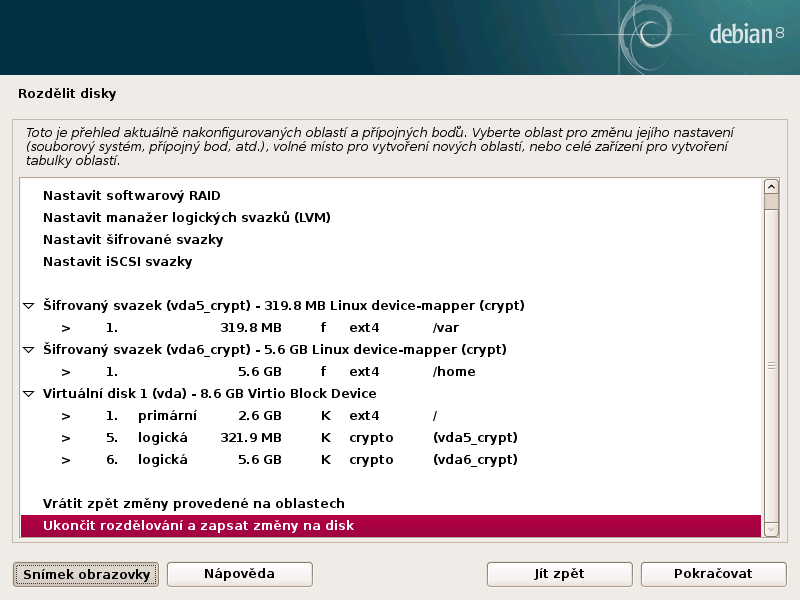
\includegraphics[width=.8\columnwidth]{pics/debian1.png}
\end{figure}

\subsection{Ubuntu}

Ubuntu linux vychází z~výše zmíněné distribuce Debian, instalátor však používá svůj vlastní. Je také jediným zástupcem linuxové distribuce, která využívá  schéma 
pro znázornění stavu rozděleného disku. Dříve využívané schéma programu GParted bylo nahrazeno jednoduchou linkou v~horní oblasti okna instalátoru. Na této lince jsou barevně znázorněny diskové 
oddíly vytvořené uživatelem. Stejné barvy jsou poté použity u~každého ze záznamů v~seznamu oddílů, jak je možné vidět na obrázku č. 2. Tento jednoduchý diagram umožňuje rychlý odhad poměrů různých 
částí, které budou vytvořeny.

\begin{figure}[b]
\label{fig:ubuntu}
\caption{Distribuce Ubuntu}
\centering
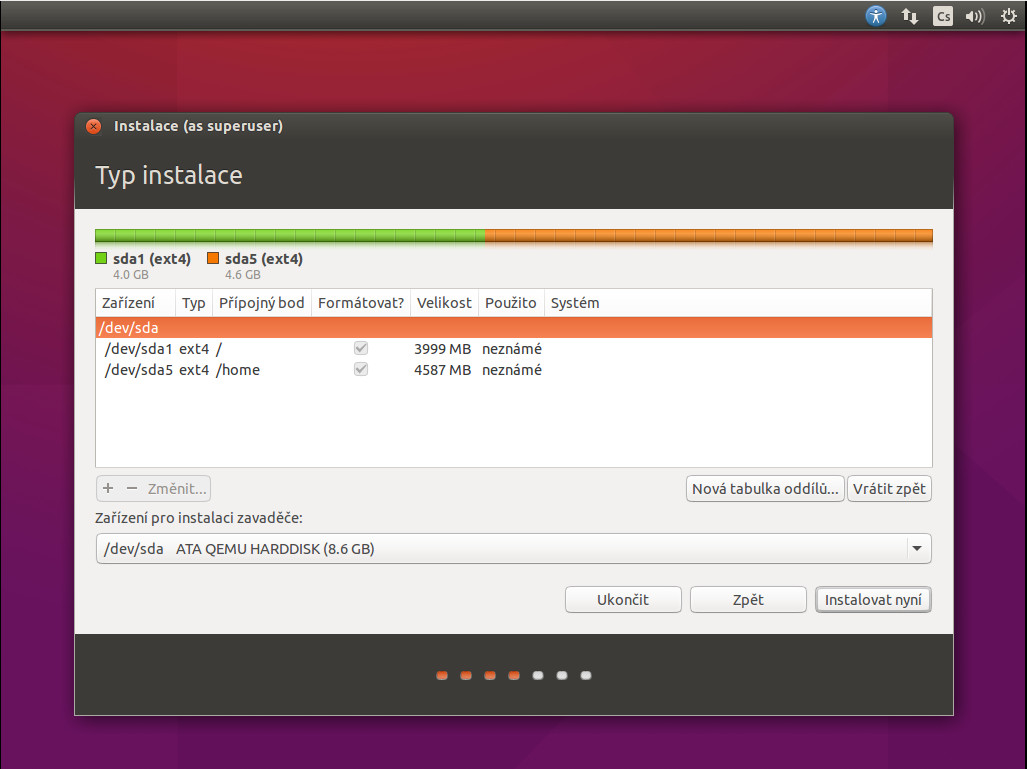
\includegraphics[width=.8\columnwidth]{pics/ubuntu1.jpg}
\end{figure}

\subsection{CentOS}

Jako příklad systémů, které využívají instalátor Anaconda jsem vybral systém CentOS. Tato zkratka znamená Community ENterprise Operating System. Na svých stránkách uvádějí \uv{The CentOS Linux
distribution is a~stable, predictable, manageable and reproducible platform derived from the sources of Red Hat Enterprise Linux (RHEL).}~\cite{CentOS} Jedná se v~podstatě o~systém Red Hat Enterprise 
Linux, ovšem bez podpory a~oprav od společnosti Red Hat. V~současné době instalátor Anaconda používá též pouze textovou reprezentaci disku. Rozdíl oproti ostatním distribucím tvoří 
seznam změn, který je zobrazen před finálním potvrzením a~započetím formátování. Na obrázcích č. 3 a~4 můžeme vidět příklad tohoto seznamu. Situaci zpřehledňuje ale pouze pro malý počet změn. Seznam s~mnoha 
záznamy o~změnách je nepřehledný. Zlepšením uživatelské přívětivosti při finální kontrole před instalací se zabývá tato práce.

\begin{figure}[hb]
\label{fig:centos1}
\caption{Distribuce CentOS}
\centering
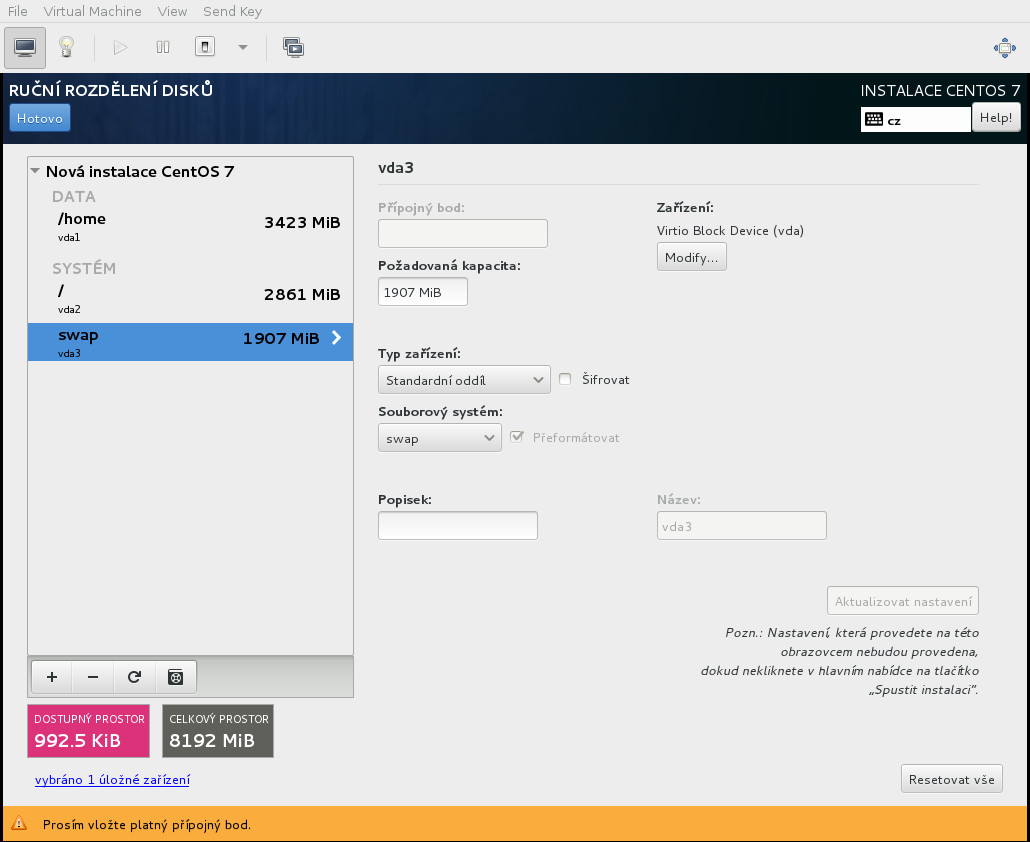
\includegraphics[width=.8\columnwidth]{pics/centos1.jpg}
\end{figure}

\begin{figure}[hb]
\label{fig:centos2}
\caption{Distribuce CentOS příklad souhrné tabulky}
\centering
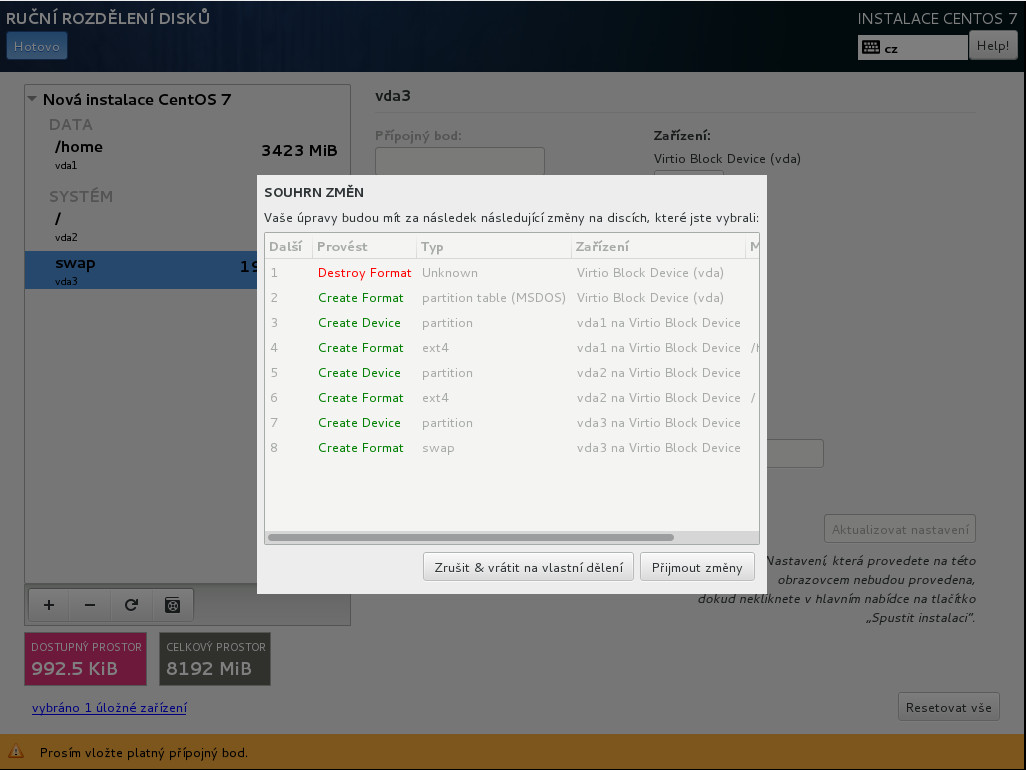
\includegraphics[width=.8\columnwidth]{pics/centos3.jpg}
\end{figure}

\subsection{Windows 10}

Pro srovnání uvádím i~příklad nejrozšířenějšího systému, Windows. Vybral jsem, v~současnosti nejnovější verzi, Windows 10. Překvapivě ani zde nejsou využity vizuální pomůcky.
Tvůrci instalátoru spoléhají na automatickou instalaci a~rozdělení disku s~tím že pokročilou verzi s~manuálním nastavováním zvolí uživatel, který se zorientuje během instalace i~bez vodítek. Předchozí verze využívají stejný systém jako má distribuce Ubuntu, tj. obdélník znázorňující disk, v~němž jsou barevně vyznačeny diskové oddíly.

\begin{figure}[h]
\label{fig:win}
\caption{Systém Windows}
\centering
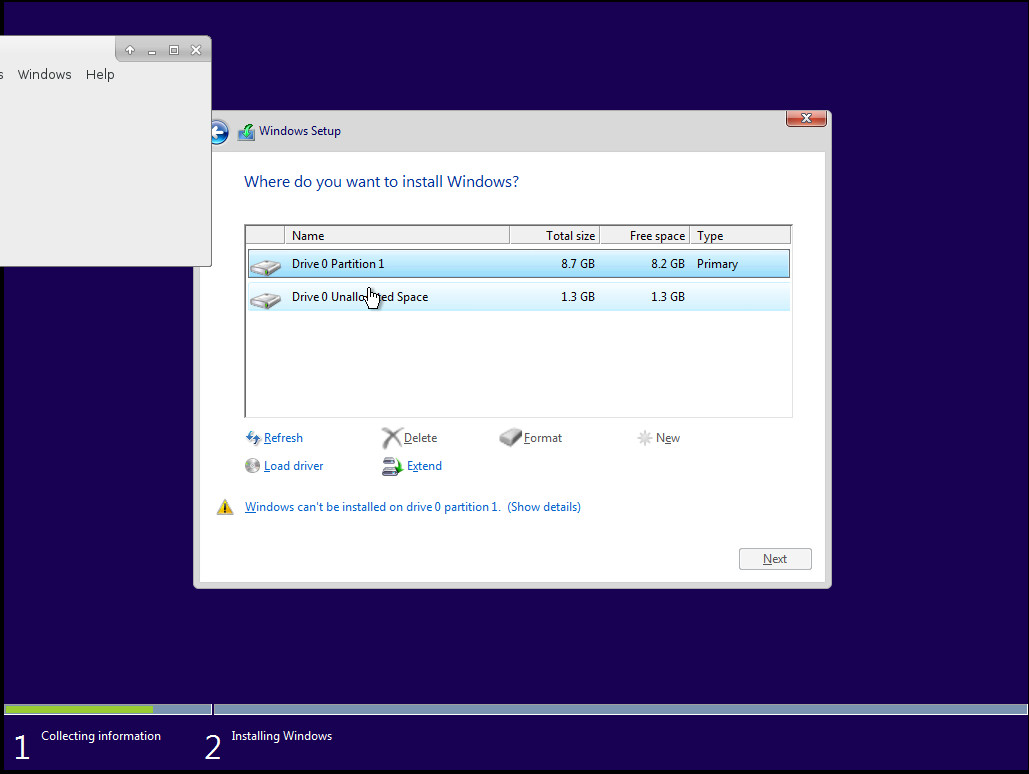
\includegraphics[width=.8\columnwidth]{pics/win1.jpg}
\end{figure}

\section{Programy sloužící pro manipulaci s~disky}

\subsection{GPatred}

Program GParted je zástupcem programů, které je možné spouštět i~mimo fázi instalace systému. Dříve byl součástí instálátoru systému Ubuntu, ale je možné jej spouštět i~samostatně, například 
 zvětšovat úložné kapacitu virtuálních disků či disků jejichž souborový systém umožňuje pozdější modifikaci. Opět je využito dříve zmíněné schéma obdélníku. Každý disk je reprezentovaný 
obdélníkem a~další informace jsou zobrazovány barevnými rámci uvnitř těchto obdélníků. Narozdíl od ostatních zmíněných programů obsahuje GParted i~grafické aplikace pro manipulaci s~disky 
a~tím dosahuje efektu WYSIWYG (What You See Is What You Get, editor, který přímo ukazuje aktuální změny) editoru. Příkladem je aplikace pro zvětšení diskového oddílu, který vidíme na obrázku č. 6.

\begin{figure}[hb]
\label{fig:gparted}
\caption{Ukázka widgetu pro program GParted~\cite{GParted}}
\centering
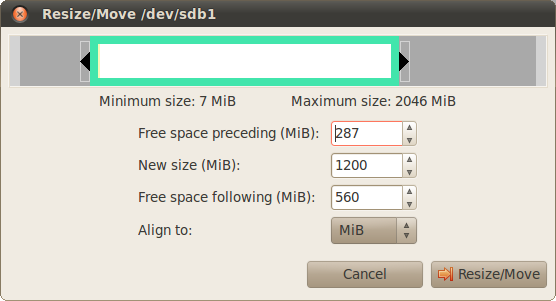
\includegraphics[width=.8\columnwidth]{pics/gparted-5-big.png}\\
\end{figure}

\subsection{Blivet-gui}

Druhým příkladem je program na manipulaci s~disky, který je součástí instalátoru Anaconda, využívá knihovnu nazvanou blivet. Knihovna blivet je základem pro všechny systémy vycházející ze systému RHEL. Autoři 
se zprvu rozhodli použít známé schéma, avšak brzy narazili na problém s~větším počtem disků včetně virtuálních. Na obrázku vidíme, že současné řešení je nedostatečné a~použití grafu by
situaci zpřehlednilo. Jednotlivé úrovně barevných rámců jsou znározněny samostatnými uzly grafu s~hranami vyznačujícími vztahy mezi nimi. 
\printbibliography

\begin{figure}[hb]
\label{fig:blivet}
\caption{Ukázka programu blivet-gui~\cite{blivet-gui}}
\centering
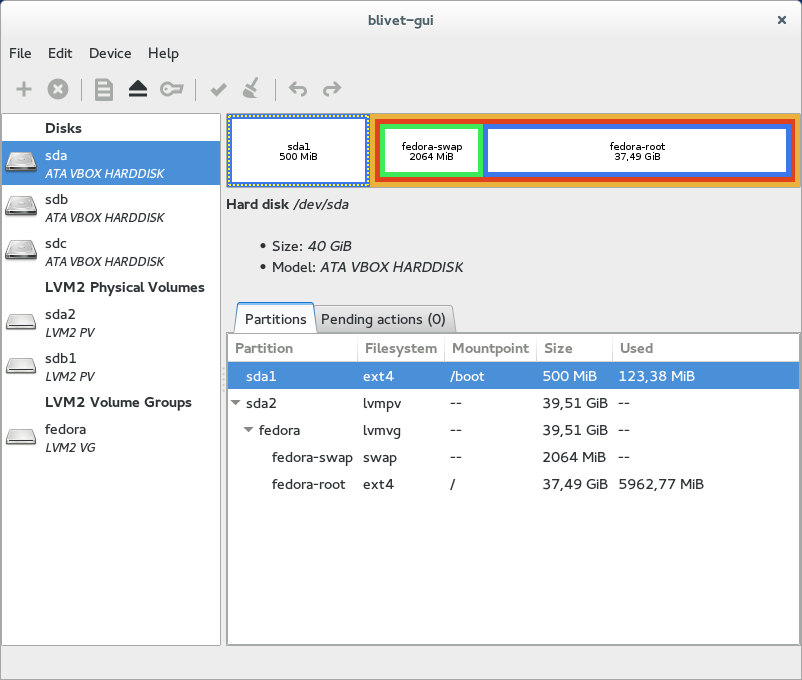
\includegraphics[width=.8\columnwidth]{pics/blivet-gui-1.png}\\
\end{figure}
\end{document}
